\chapter{Hinführung zum Thema}

\section{Thema der Arbeit}
In der vorliegenden Arbeit werden Einflussfaktoren auf den Kurs von ausgewählten Kryptowährungen gesucht und der Grad des Einflusses evaluiert. Dies geschieht mit dem Ziel herauszufinden, ob sich die Kursschwankungen der digitalen Währungen voraussagen lassen und wenn ja, in welchem Maße. Im nachfolgenden Kapitel wird auf die Motivation hinter der Analyse eingegangen. Das genaue Vorgehen und die Ziele werden wird in Abschnitt \ref{chapter:Vorgehen} erläutert.

\section{Bitcoin als Vorreiter der Krypotowährungen}
Geld online von einem Teilnehmer direkt zu einem Anderen senden, ohne dabei (Transaktions-)Gebühren für einen zwischengelagerten Finanz-Dienstleister zahlen zu müssen, ist der Gedanke hinter dem "Peer-To-Peer Electronic Cash System"\citep{nakamoto_bitcoin:_2008} Bitcoin. Obwohl es Teilnehmern ohne Aufwand möglich ist, dem Netzwerk beizutreten oder es wieder zu verlassen, ist es solange unangreifbar, solange ein Angreifer nicht dauerhaft über mehr Rechenkapazität verfügt, als das komplette restliche Netzwerk.\citep{nakamoto_bitcoin:_2008} Ob das Bitcoinnetzwerk wirklich absolute Anonymität gewährt, wird stark kritisiert.\citep{reid_analysis_2013,androulaki_evaluating_2013}. In der Tat werden beim Nutzen des Netzwerk jedoch keine persönlichen Informationen an ein Kreditinstitut (wie PayPal, Paydirekt, ApplePay oder Masterpass) weitergegeben. Diese Argumente (Kostenreduktion, Sicherheit und Anonymität) sorgen für Interesse an der digitalen Währung (auch hier gibt es Kritiker, die den Bitcoin als Investition und nicht als Währung bezeichnen)\citep{baur_bitcoin:_2015}. Nicht zu vernachlässigen ist an dieser Stelle auch das Interesse der Industrie an "Smart Contracts"\citep[S.~10]{dannen_introducing_2017}, die beispielsweise im Bereich des Internet of Things Anwedung finden.\citep{christidis_blockchains_2016}\newline
Neben Bitcoin hat sich deshalb zusätzlich eine Vielzahl an anderen sogenannten Kryptowährungen entwickelt. Die Währungen mit dem größten Marktvolumen sind  Bitcoin(\ref{subsec:Bitcoin}) und Ethereum(\ref{subsec:Ethereum})\citep{wood_ethereum:_2014}.\citep{brandt_infografik:_2017, coinmarketcap_ranking_2017} Daneben gibt es noch sogenannte Altcoins (aus dem Englischen: alternative coin\citep{prableen_bajpai_altcoin_2014})(\ref{subsec:Altcoins}). Mittlerweile umfassen diese 664 Bitcoin-Alternativen.\citep{coindesk_anzahl_2017}. Obgleich die tatsächliche Nutzung der Krypowährungen sehr gering ist (1\% der Befragten in Deutschland\citep{tsys_kennen_2016}), steigt das Interesse an Kryptowährungen\citep{wikitrends_compare_2017,googletrends_googletrends_2017}.\newline
\todo{irgendwas zu Technik später oder so?}

\section{Machine Learning, Data Mining, Data Analysis und Data Science}
Die Themen Machine Learning, Data Mining, Data Analysis und Data Science sind verwandte Begriffe aus dem interdisziplinären Bereich der Statistik und Informatik.  \newline
Der Begriff Machine Learning gehört in der Informatik und Mathematik zur Familie der Künstlichen Intelligenz.\multicitep{kim_matlab_2017, S.~2; swamynathan_mastering_2017, S.~54}. Es kann als "Sammlung von Algorithmen und Techniken" verstanden werden, die "genutzt werden, um Computersysteme zu erstellen, die aus Daten lernen, um Vorhersagen zu erstellen".\citep[S.~53; eigene Übersetzung]{swamynathan_mastering_2017} Bekannte Anwendungen aus dem Alltag sind Empfehlungssysteme oder Spamerkennungen.\citep[S.~53]{swamynathan_mastering_2017}\newline
Data Mining beschreibt den Prozess, aus einer gewaltigen Menge an Daten die "richtigen Daten", zur "richtigen Zeit" für die "richtigen Entscheidungen"\citep[S.~61; eigene Übersetzung]{swamynathan_mastering_2017} zu gewinnen. Für diesen Prozess haben sich im Laufe Zeit drei Frameworks herauskristallisiert\citep[p.69]{swamynathan_mastering_2017}:
\begin{itemize}
\item Knowledge Discovery Databases (KDD) process model
\item CRoss Industrial Standard Process for Data Mining (CRISP – DM)
\item Sample, Explore, Modify, Model and Assess (SEMMA)
\end{itemize}
Neben Schnittmengen mit Künstlicher Intelligenz, Machine Learning und der Statistik, befasst Data Mining sich ebenfalls mit Datenbanksystemen.\citep[S.~4]{ramasubramanian_machine_2017} \newline
Eng verwandt mit dem Data Mining ist die Datenanalyse (engl. Data Analysis; in der Industrie auch Business Analytics\citep[S.~58]{swamynathan_mastering_2017}). Sie wird benutzt um\citep[S.~2]{hertle_datenanalyse_2016}
\begin{enumerate}
\item Messdaten zu verstehen,
\item Gesetzmäßigkeiten zu extrahieren und
\item die Zukunft vorherzusagen.
\end{enumerate}
Dazu bedient sie sich der deskriptiven Statistik, der explorativen Datentenanalyse (engl. Explorative Data Analysis; EDA) und der Induktiven Statistik.\citep[S.~17]{hertle_datenanalyse_2016}\newline
Um 
\begin{itemize}
\item den Anstieg der Datenmengen in der Datenanalyse,
\item die Veränderung im Aussehen der Daten (unstrukturiert oder semi-strukturiert statt strukturiert) und
\item die Wandlung Semantik der zugrundeliegenden Daten (Daten liegen in Markup-Sprachen vor und enthalten zusätzliche Informationen)
\end{itemize}
darzustellen, hat sich der Begriff Data Science entwickelt.\citep{dhar_data_2013} Er versucht die geänderten Anforderungen der heutigen Datenanalyse abzubilden (siehe \ref{fig:dataEvolution}).
\begin{figure}[h]
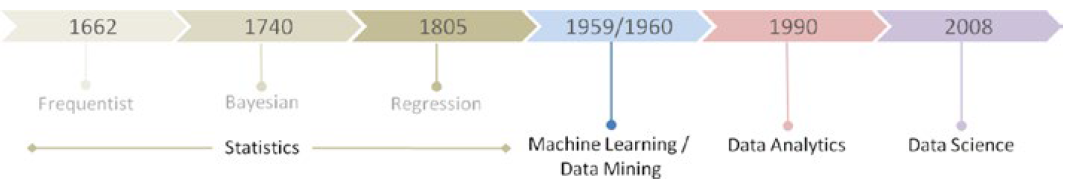
\includegraphics[width=\textwidth]{images/LearnFromDataEvolution.png}
\caption{Learn from data evolution \citep[p.66]{swamynathan_mastering_2017}}
\label{fig:dataEvolution}
\centering
\end{figure}
\newline
Wie anfänglich erwähnt, sind alle genannten Begriffe miteinander verwandt. Das Gewinnen von Erkenntnissen aus Daten, um beispielsweise die Zukunft vorherzusagen, nennt sich Data Analysis. Werden die Daten aus verschiedensten Datenbanken oder Datawarehouses gewonnen, spricht man von Data Mining. Handelt es sich dabei noch um Informationen unterschiedlicher Struktur und große Datensätze, so befindet man sich im Bereich der Data Science. Der inhärente Erkenntnisgewinn dieser Verfahren kann von von menschlicher Seite kommen oder durch Machine Learning geschehen.\newline
Verdeutlicht wird dies durch Projekte wie Googles DeepMind\citep{deepmind_technologies_limited_deepmind_2017}, IBMs Watson\citep{international_business_machines_corporation_ibm_ibm_2017} oder Sprachassistenten wie Siri, Alexa und Bixby. Sie zeigen, dass großes Interesse an Machine Learning und Data Science herrscht. Deshalb haben sich auch ganze Berufsfelder wie "machine learning engineer", "data engineer" oder "data scientist"\citep[S.~1]{ramasubramanian_machine_2017} gebildet.



\section{Cloud-Dienste und SaaS}
Cloud Computing beschreibt "ein Modell, das es erlaubt bei Bedarf, jederzeit und überall bequem über ein Netz auf einen geteilten Pool von konfigurierbaren Rechnerressourcen (z. B. Netze, Server, Speichersysteme, Anwendungen und Dienste) zuzugreifen, die schnell und mit minimalem Managementaufwand oder geringer ServiceproviderInteraktion zur Verfügung gestellt werden können"\citep[S.~18]{appelrath_future_2014-1}. Innerhalb des Cloud Computing unterscheidet man weiterhin zwischen verschiedenen Cloud-Diensten (engl. cloud services). Nach \citep[S.~20]{appelrath_future_2014-1} differenziert man zwischen den Services in \ref{tab:CloudServices}.
\begin{table}[h]
\begin{tabular}{|p{5cm}|p{10cm}|}
\hline
\hline
\textbf{Diensttyp} & \textbf{Beschreibung}\\
\hline
Infrastructure as a Service (IaaS) & Virtuelle Hardware oder Infrastruktur, zum Beispiel Speicherplatz, Rechenleistung oder Netzwerkbandbreite\\
\hline
Platform as a Service (PaaS) & Programmierframeworks, Bibliotheken und Werkzeuge, um Anwendungen unter eigener Kontrolle auf
Cloud-Infrastrukturen bereitstellen zu können, ohne die zugrunde liegende Infrastruktur wie Netzwerk,
Server, Betriebssysteme oder Speicher managen oder kontrollieren zu müssen\\
\hline
Software as a Service (SaaS) & Vollständige Anwendungen, die auf Cloud-Infrastrukturen betrieben und beispielsweise über einen
Webbrowser aufrufbar sind, wobei Nutzer weder die zugrunde liegende Cloud-Infrastruktur noch
individuelle Anwendungseinstellungen (mit der möglichen Ausnahme der eingeschränkten Konfiguration
von Nutzereinstellungen) kontrollieren müssen und können\\
\hline
Mashup as a Service (MaaS) & Verknüpfung einzelner Software-Komponenten (unter anderem auch Cloud-Dienste) zu einem aggregierten
Cloud-Dienst\\
\hline
Business Process as a Service (BPaaS) & Konkrete Geschäftsanwendungen (beispielsweise CRM) als Verknüpfung einzelner Software-Komponenten
(standardisierte MaaS)\\
\hline
\end{tabular}
\caption{Cloud-Diensttypen}
\label{tab:CloudServices}
\end{table}
\citep[P.~23]{appelrath_future_2014-1} sprechen generell von "Cloud Computing als disruptiver Innovationsfaktor". An dieser Stelle wird besonders Software as a Service betrachtet. Dort stieg der Umsatz von 10,75 Mrd. USD im Jahr 2010 auf 38,57 Mrd. USD im Jahr 2016. Für die Zukunft (2020) wird sogar ein Umsatz von 75,73 Mrd. USD prognostiziert.\citep{gartner_umsatz_2017} Das ist eine Steigerung von über 700\% in nur 10 Jahren. Dies kann einerseits durch offensichtliche Vorteile, wie "höhere Stabilität und Planungssicherheit", der "Möglichkeit Anwender schnell ins System einzuführen" und "Erschließung neuer Kundengruppen"\citep{fraunhofer_vorteile_2010} erklärt werden, andererseits aber auch durch Tendenz der Softwarebranche hin zur serviceorientierten Architekturen (engl. service oriented atchitekture; SOA).\citep[P.~22]{appelrath_future_2014-1} Dieser Trend zu SaaS kann beobachtet werden, wenn reine Cloud-Anbieter wie Salesforce "klassische" Anbieter wie SAP den Rang als "Spitze des Weltmarkts der Software für Customer Relationship Management (CRM)"\citep{fritsch_salesforce.com_2013} ablaufen.\newline
Laut einer Studie von \citep{bitkom_welche_2017} greifen 23\% der befragten Unternehmen in Deutschland neben "Office Anwendungen aus der Cloud", "Security as a Service" und "Groupware" auf "Business Intelligence/Big Data"-Software aus der Cloud zurück. Zu dieser Kategorie gehört auch Azure Machine Learning (kurz: Azure ML) von Microsoft, welches zur Analyse in dieser Arbeit verwendet wird.